\subsection{Controller Fusion Diagnostics}
\label{sec:controller-diagnostics}

To evaluate the semantic precision and interpretability of controller integration, we analyze three distinct injection mechanisms: (1) prefix token interpolation, (2) additive attention biasing, and (3) gated residual modulation. Each scheme receives identical controller input \(\tilde{s}\), formed via:
\[
\tilde{s} = \sum_{k=1}^K \alpha_k s_k, \quad \alpha_k = \frac{\exp(w_k)}{\sum_{\ell=1}^K \exp(w_\ell)}.
\]

Let \(\mathcal{F}_m(\cdot, \tilde{s})\) denote the model with injection mode \(m \in \{\mathrm{prefix}, \mathrm{bias}, \mathrm{gate}\}\). For fixed input \(x\), we study the perturbation and propagation effects caused by controller fusion.

\subsubsection*{Injection Influence}

We define influence magnitude as the \(L_2\) norm of the difference in output logits between the controller-injected and controller-ablated models:
\[
\Delta^{(m)}(x) = \left\| \mathcal{F}_m(x, \tilde{s}) - \mathcal{F}_m(x, \mathbf{0}) \right\|_2.
\]

This is computed layerwise to identify zones of concentrated influence and injection saturation. Stronger deviations at higher layers imply delayed controller fusion, whereas front-loaded shifts suggest syntactic modulation.

\begin{figure}[H]
  \centering
  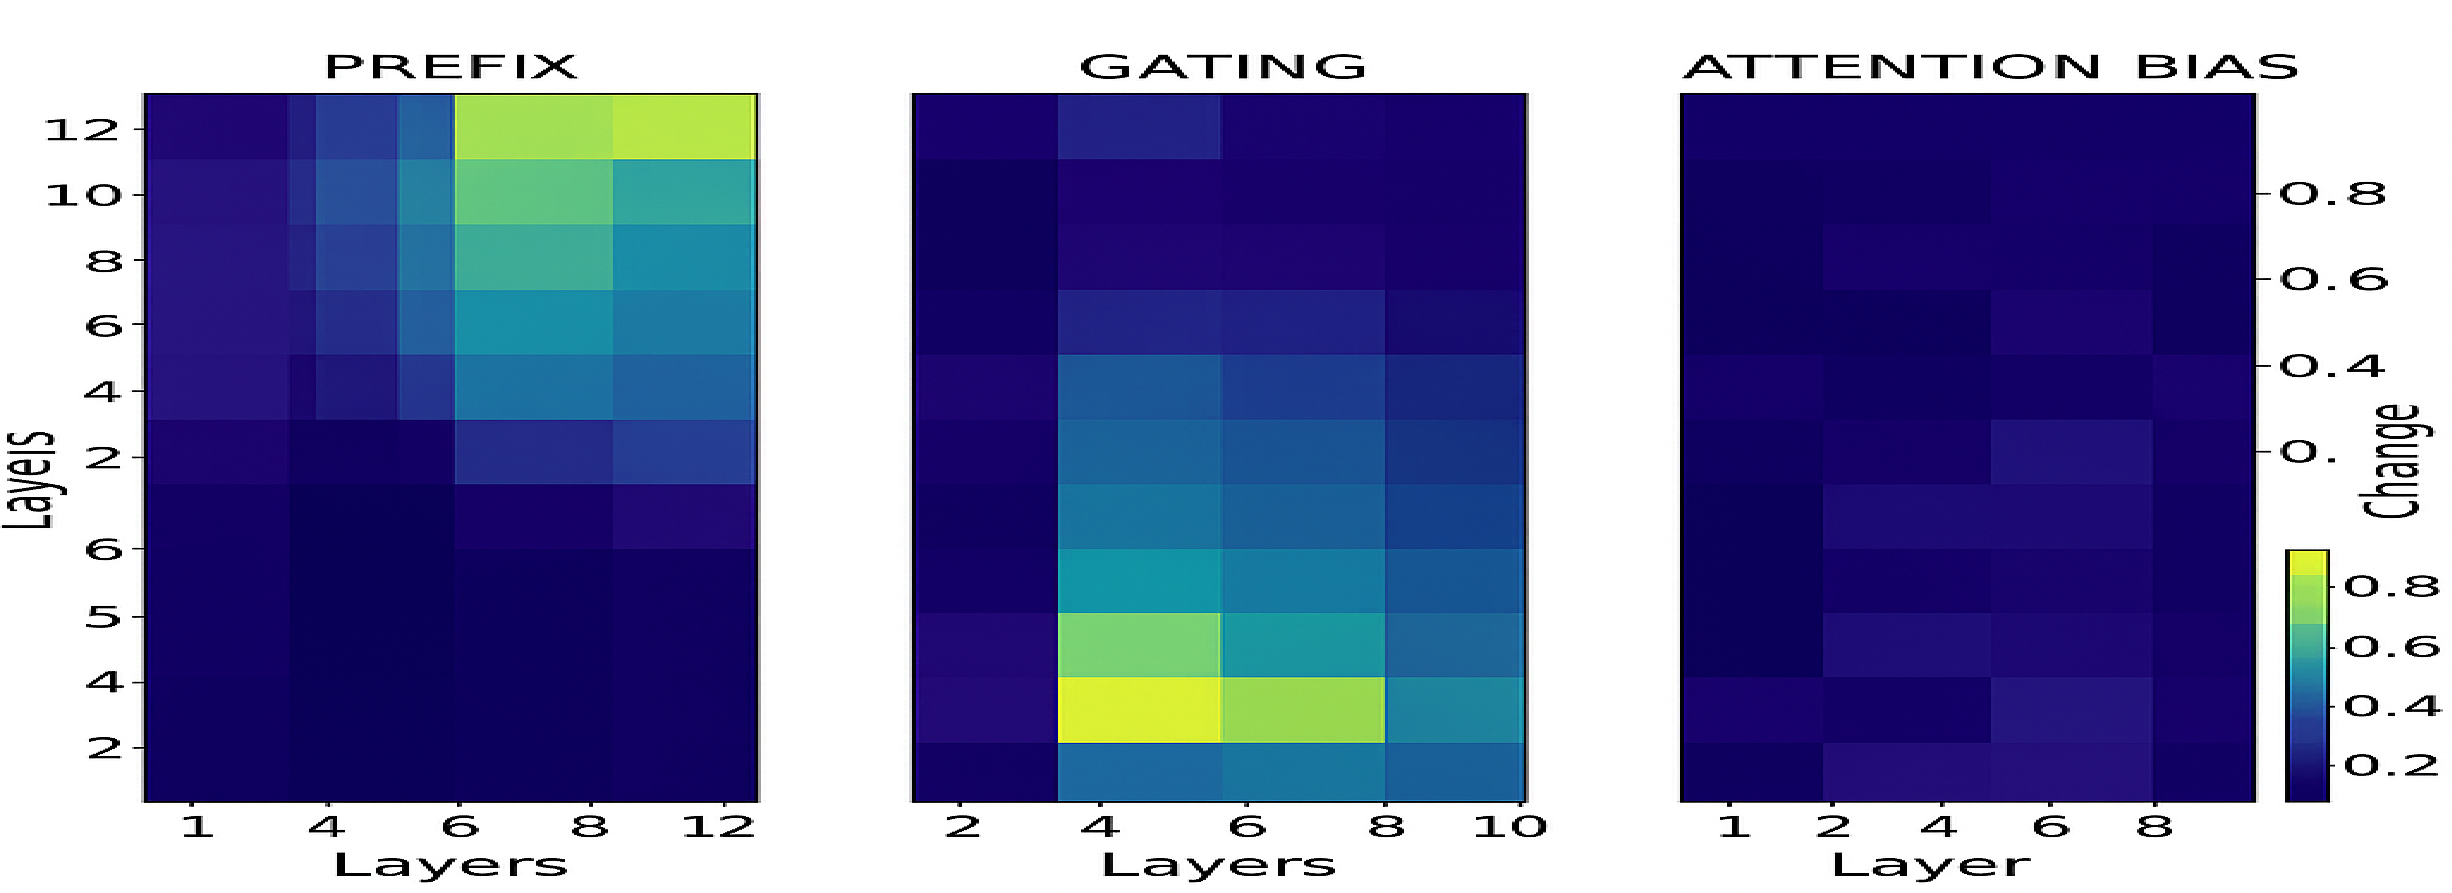
\includegraphics[width=\textwidth]{figures/figure_7.png}
  \caption{Layerwise controller influence heatmap across injection modes. Prefix tuning shifts early logits; gating modulates mid-depth; attention bias generates scattered low-intensity changes.}
  \label{fig:controller_comparison}
\end{figure}

\subsubsection*{Layerwise Traceability}

For each mode, we analyze the cross-attention matrix \(A_\ell \in \mathbb{R}^{T \times T}\) for layer \(\ell\) with and without controller conditioning. We compute the Frobenius deviation:
\[
\delta_\ell^{(m)} = \left\| A_\ell^{(\tilde{s})} - A_\ell^{(\mathbf{0})} \right\|_F.
\]
This reflects how controller information realigns global attention. Qualitative visualizations of \(A_\ell\) reveal syntactic shifts in focal connectivity—e.g., subject-verb alignment influenced by downstream semantic intent.

\subsubsection*{Mode Disambiguation}

To quantify controller disambiguation across routing paths, we measure variance between induced representations under different interpolation vectors \(\tilde{s}^{(1)} \ne \tilde{s}^{(2)}\), derived from two distinct span combinations \(S^{(1)}, S^{(2)}\). Let \(h_{\text{final}}^{(m, i)}\) be the layer \(L\) hidden state under controller vector \(\tilde{s}^{(i)}\) with mode \(m\), then:
\[
\mathrm{D}_{\text{route}}^{(m)} = \mathbb{E}_{x \sim \mathcal{D}} \left[ \left\| h_{\text{final}}^{(m, 1)}(x) - h_{\text{final}}^{(m, 2)}(x) \right\|_2 \right].
\]

A higher \(\mathrm{D}_{\text{route}}^{(m)}\) implies that controller fusion more effectively channels distinct routing hypotheses into separable downstream representations.

\vspace{0.75em}
\noindent\textbf{Gated Probe Interventions.} Following the probing methodology in \cite{vig2020investigating}, we optionally perform controller swap experiments:
\[
\tilde{s}_{\text{content}} \leftarrow \tilde{s}_{\text{confound}}, \quad \text{while keeping } x \text{ fixed}.
\]
This tests whether the model's behavior aligns more with structural routing or surface-level tokens, revealing how \(\tilde{s}\) perturbs token importance.

\begin{proposition}[Disentanglement under Orthogonal Controllers]
\label{prop:orthogonal_fusion}
Let \(\tilde{s}^{(1)}, \tilde{s}^{(2)} \in \mathbb{R}^d\) be orthogonal controller vectors such that \(\langle \tilde{s}^{(1)}, \tilde{s}^{(2)} \rangle = 0\), and let the layer \(\ell\) hidden state be modulated by additive controller fusion:
\[
h^\ell = f(x^\ell) + W_m^\ell \tilde{s},
\]
where \(W_m^\ell \in \mathbb{R}^{d' \times d}\) is the injection weight matrix for fusion mode \(m\), and \(f(\cdot)\) is the controller-independent component. Assume the final output logits are computed via a linear decoder:
\[
\mathcal{F}_m(x, \tilde{s}) = V h^L,
\]
where \(V \in \mathbb{R}^{C \times d'}\) projects to logits over \(C\) classes. If \(W_m^\ell\) is full rank and \(V W_m^\ell\) has spectral norm bounded below by \(\sqrt{\epsilon} > 0\), then:
\[
\left\| \mathcal{F}_m(x, \tilde{s}^{(1)}) - \mathcal{F}_m(x, \tilde{s}^{(2)}) \right\|_2^2 \geq \epsilon \cdot \left\| \tilde{s}^{(1)} - \tilde{s}^{(2)} \right\|_2^2.
\]
\end{proposition}

\begin{proof}
\textbf{Step 1:} Express the difference in output logits.
We compute the difference in output logits:
\[
\Delta := \mathcal{F}_m(x, \tilde{s}^{(1)}) - \mathcal{F}_m(x, \tilde{s}^{(2)}) = V W_m^\ell (\tilde{s}^{(1)} - \tilde{s}^{(2)}).
\]

\textbf{Step 2:} Compute the squared norm.
By the definition of the operator norm:
\[
\|\Delta\|_2^2 = \left\| V W_m^\ell (\tilde{s}^{(1)} - \tilde{s}^{(2)}) \right\|_2^2.
\]

\textbf{Step 3:} Apply the norm inequality for linear transformations.
Since \(V W_m^\ell\) is a linear map from \(\mathbb{R}^d \to \mathbb{R}^C\), and \(\tilde{s}^{(1)} - \tilde{s}^{(2)}\) lies in \(\mathbb{R}^d\), we apply the norm inequality for linear transformations:
\[
\| \Delta \|_2^2 \geq \sigma_{\min}^2 \cdot \left\| \tilde{s}^{(1)} - \tilde{s}^{(2)} \right\|_2^2,
\]
where \(\sigma_{\min}\) is the smallest singular value of \(V W_m^\ell\).

\textbf{Step 4:} Apply the spectral norm assumption.
By assumption, \(V W_m^\ell\) is full-rank and has minimal singular value at least \(\sqrt{\epsilon}\), so:
\[
\sigma_{\min}(V W_m^\ell) \geq \sqrt{\epsilon}.
\]

\textbf{Step 5:} Conclude the bound.
Therefore:
\[
\| \Delta \|_2^2 \geq \epsilon \cdot \left\| \tilde{s}^{(1)} - \tilde{s}^{(2)} \right\|_2^2.
\]
This completes the proof.
\end{proof}

